\id{МРНТИ 61.37.35}{https://doi.org/10.58805/kazutb.v.2.27-930}

\begin{articleheader}
\sectionwithauthors{З.М. Молдахметов, С.Д. Фазылов, О.A. Нуркенов, А.Ж. Сарсенбекова, И.А. Пустолайкина, Ж.Б. Сатпаева, Р.E. Бакирова, Ж.С. Нурмаганбетов, А.К. Сыздыков}{МОЛЕКУЛЯРНОЕ МОДЕЛИРОВАНИЕ И ТЕРМОХИМИЧЕСКИЕ СВОЙСТВА КОМПЛЕКСОВ ВКЛЮЧЕНИЯ ГИДРАЗОНОВ ГИДРОКСИЗАМЕЩЕННЫХ БЕНЗОЙНЫХ КИСЛОТ С ЦИКЛОДЕКСТРИНАМИ}

{\bfseries
\textsuperscript{1}З.М. Молдахметов\alink{https://orcid.org/0000-0001-9497-2545},
\textsuperscript{1}С.Д. Фазылов\textsuperscript{\envelope }\alink{https://orcid.org/0000-0002-4240-6450},
\textsuperscript{1}О.A. Нуркенов\alink{https://orcid.org/0000-0003-1878-2787;},
\textsuperscript{2}А.Ж. Сарсенбекова\alink{https://orcid.org/0000-0002-8951-3616},
\textsuperscript{2}И.А.~Пустолайкина\alink{https://orcid.org/0000-0001-6319-666X},
\textsuperscript{2}Ж.Б. Сатпаева\alink{https://orcid.org/0000-0003-0962-1148},
\textsuperscript{3}Р.E. Бакирова\alink{https://orcid.org/0000-0002-1592-8579},
\textsuperscript{1}Ж.С. Нурмаганбетов\alink{https://orcid.org/0000-0002-0978-5663},
\textsuperscript{4}Г.Н.Мусина\alink{https://orcid.org/0009-0008-1280-2648},
\textsuperscript{1}А.К.~Сыздыков\alink{https://orcid.org/0000-0002-1592-8579}
}
\end{articleheader}

\begin{affiliation}
\textsuperscript{1}Институт органического синтеза и углехимии, Караганда, Казахстан,

\textsuperscript{2}Карагандинский университет им. Е.А. Букетова, Караганда, Казахстан,

\textsuperscript{3}Медицинский университет Караганды, Казахстан,

\textsuperscript{4}Карагандинский технический университет им. А.Сагинова, Караганда, Казахстан

\raggedright \textsuperscript{\envelope }Корреспондент-автор: e-mail: iosu8990@mail.ru
\end{affiliation}

В представленной работе методами молекулярного докинга и моделирования
выполнено \emph{in silico} изучение и рассмотрены механизмы образования
клатратных комплексов включения 2- и 4-гидрок\-сигидразидов бензойных
кислот и их гидразонов с циклодекстринами (α-, β-, γ-циклодекстринов).
Методом молекулярного докинга, с целью выбора наиболее эффективного
комплексообразующего агента из трех циклодекстринов, было выполнено
исследование комплексообразующих особенностей двух молекул для системы
циклодекстрин-гидразон с равномолярным молярным соотношением. Все
исследуемые гидразоны продемонстрировали наилучшее значение афинности
связывания с β-циклодекстрином. Эффективность связывания исследуемых
гидразонов с циклодекстринами обеспечивается прежде всего соответствием
геометрических параметров связывающихся молекул, образующих единую
клатратную систему. Комплексообразование 2- и 4-гидроксигидразидов
бензойных кислот и их гидразонов c циклодекстринами протекает участием
как внутренних Н3 и Н5 протонов циклодекстриновой полости, так и
расположенных на внешней поверхности их конического конуса с
образованием смешанных водорастворимых клатратных соединений.
Соотношение геометрических параметров молекул 2- и 4-гидразидов
бензойных кислот и их гидразонов с размерами полостей молекул α-, β- и
γ-циклодекстринов, позволяет предположить возможность образования ими
клатратных комплексов. Предложенные в работе оптимальные условия
инкапсулирования гидразоновых производных бензойной кислоты
олигосахаридами могут быть использованы при получении водорастворимых
форм аналогичных соединений.

{\bfseries Ключевые слова}: афиннность связывания, циклодекстрин,
клатратный комплекс, гидразон, термографический анализ.

\begin{articleheader}
{\bfseries ГИДРОКСИАУЫСҚАН БЕНЗОЙ ҚЫШҚЫЛДАРЫНЫҢ ТҰЙЫҚДЕКСТРИНДЕРМЕН КЕШЕНДІ ҚОСЫЛЫСТАРЫНЫҢ МОЛЕКУЛАЛЫҚ МОДЕЛДЕЛУІ ЖӘНЕ ТЕРМОХИМИЯЛЫҚ ҚАСИЕТТЕРІ}

{\bfseries
\textsuperscript{1}З.М. Молдахметов,
\textsuperscript{1}С.Д. Фазылов\textsuperscript{\envelope },
\textsuperscript{1}О.A. Нүркенов,
\textsuperscript{2}А.Ж. Сарсенбекова,
\textsuperscript{2}И.А. Пустолайкина,
\textsuperscript{2}Ж.Б. Сатпаева,
\textsuperscript{3}Р.E. Бакирова,
\textsuperscript{1}Ж.С. Нұрмағанбетов,
\textsuperscript{1}А.К. Сыздықов
}
\end{articleheader}

\begin{affiliation}
\textsuperscript{1}Органикалық синтез және көмірхимиясы институты, Қарағанды, Қазақстан,

\textsuperscript{2} Е.А. Букетов атындағы Қарағанды университеті, Қарағанды, Қазақстан,

\textsuperscript{3}Қарағанды медицина университеті, Қарағанды, Қазақстан,

\textsuperscript{4}Ә.Сағынов атындағы Қарағанды техникалық университеті, Қарағанды, Қазақстан,

e-mail: iosu8990@mail.ru
\end{affiliation}

Ұсынылған жұмыста молекулярлық қондыру және модельдеу әдістерін қолдана
отырып, \emph{in silico} зерттеу жүргізілді және бензой қышқылдарының 2-
және 4-гидроксигидразидтерінің клатратты инклюзия кешендерінің және
олардың циклодекстриндерімен (α-, β-, γ-циклодекстриндер)
гидразондарының түзілу механизмдері қарастырылды. Молекулярлық қондыру
әдісін қолдана отырып, үш циклодекстриннің ішінен ең тиімді комплекс
түзетін агентті таңдау үшін эквимолярлы молярлық қатынасы бар
циклодекстрин-гидразон жүйесі үшін екі молекуланың комплекс түзу
қасиеттеріне зерттеу жүргізілді. Барлық зерттелген гидразондар
β-циклодекстринмен байланысуының ең жақсы мәнін көрсетті. Зерттелетін
гидразондардың циклодекстриндермен байланысуының тиімділігі ең алдымен
біртұтас клатрат жүйесін құрайтын байланыстырушы молекулалардың
геометриялық параметрлерінің сәйкестігімен қамтамасыз етіледі. Бензой
қышқылдарының 2- және 4-гидроксигидразид\-терінің және олардың
гидразондарының циклодекстриндермен комплекстенуі циклодекстрин қуысының
ішкі Н3 және Н5 протондарының және олардың конустық конусының сыртқы
бетінде орналасқан аралас суда еритін клатрат қосылыстарының түзілуімен
жүреді. Бензой қышқылдарының 2- және 4-гидразидтерінің және олардың
гидразондарының молекулаларының геометриялық параметрлерінің α-, β- және
γ-циклодекстриндер молекулаларының қуыстарының өлшемдеріне қатынасы
олардың клатраттық комплекс түзілу мүмкіндігін болжауға мүмкіндік
береді. Жұмыста ұсынылған бензой қышқылының гидразон туындыларын
олигосахаридтермен инкапсуляциялаудың оңтайлы шарттарын ұқсас
қосылыстардың суда еритін формаларын алу үшін пайдалануға болады.

{\bfseries Түйін сөздер:} байланысу афиндігі, тұйықдекстрин, клатратты
кешен, гидразон, термографиялық талдау.

\begin{articleheader}
{\bfseries MOLECULAR MODELLING AND THERMOCHEMICAL PROPERTIES OF INCLUSION COMPLEXES OF HYDROXY-SUBSTITUTED BENZOIC ACIDS HYDRAZONES WITH CYCLODEXTRINS}

{\bfseries
\textsuperscript{1}Z.M. Muldakhmetov,
\textsuperscript{1}C.D. Fazylov\textsuperscript{\envelope },
\textsuperscript{1}O.A. Nurkenov,
\textsuperscript{2}A.Zh. Sarsenbekova,
\textsuperscript{2}I.A. Pustolaikina,
\textsuperscript{2}J.B.~Satpayeva,
\textsuperscript{3}R.E. Bakirova,
\textsuperscript{1}Zh.S. Nurmaganbetov,
\textsuperscript{1}A.K. Syzdykov
}
\end{articleheader}

\begin{affiliation}
\textsuperscript{1}Institute of Organic Synthesis and Coal Chemistry, Karaganda, Kazakhstan,

\textsuperscript{2}E.A.Buketov University of Karaganda, Kazakhstan,

\textsuperscript{3}Medical University of Karaganda, Karaganda, Kazakhstan,

\textsuperscript{4}A.Saginov Karaganda technical university, Karaganda, Kazakhstan

e-mail: iosu8990@mail.ru
\end{affiliation}

In the presented work, the methods of molecular docking and modeling
were used to study in silico and consider the mechanisms of formation of
clathrate inclusion complexes of 2- and 4-hydroxyhydrazides of benzoic
acids and their hydrazones with cyclodextrins (α-, β-, γ-cyclodextrins).
The method of molecular docking was used to study the complexing
features of two molecules for the cyclodextrin-hydrazone system with an
equimolar molar ratio in order to select the most effective complexing
agent from three cyclodextrins. All the studied hydrazones demonstrated
the best value of binding affinity with β-cyclodex\-trin. The efficiency
of binding of the studied hydrazones with cyclodextrins is ensured
primarily by the correspondence of the geometric parameters of the
binding molecules forming a single clathrate system. Complexation of 2-
and 4-hydroxyhydrazides of benzoic acids and their hydrazones with
cyclodextrins occurs with the participation of both internal H3 and H5
protons of the cyclodextrin cavity and those located on the external
surface of their conical cone with the formation of mixed water-soluble
clathrate compounds. The ratio of the geometric parameters of the
molecules of 2- and 4-hydrazides of benzoic acids and their hydrazones
with the sizes of the cavities of the molecules of α-, β- and
γ-cyclodextrins allows us to assume the possibility of their formation
of clathrate complexes. The optimal conditions for the encapsulation of
hydrazone derivatives of benzoic acid by oligosaccharides proposed in
the work can be used to obtain water-soluble forms of similar compounds.

{\bfseries Keywords}: binding activity, cyclodextrin, clathrate complex,
hydrazone, thermographic analysis.
\vspace{-1em}
\begin{multicols}{2}
{\bfseries Введение.} Гидразоновые производные бензойной кислоты обладают
высокой биологической активностью, что стимулирует постоянный поиск и
синтез их новых производных {[}1{]}. Фрагмент «гидразид-гидразон»
присутствуют в структурном ряду многих лекарственных препаратов,
нашедших широкое применение в медицинской практике, как
антибактериальные {[}2,3{]}, противотуберкулезные {[}4{]},
aнтималярийные {[}4{]}, противовоспалительные средства {[}5{]}. Такой
широкий спектр гидразоновых соединений вызывает интерес, как к
разработке методов синтеза, так и к закономерностям количественного
соотношения структура--активность. Среди биологических свойств этого
класса соединений антибактериальная {[}2,6{]} активность является
наиболее часто встречающейся в научной литературе. Привлекательность
гидразид-гидразонов как биоактивных соединений обусловлена
многогранностью их реакционной способности, а также практическим
использованием их производных в качестве «\emph{строительных-блоков}» в
создании новых биоактивных средств и технических реагентов {[}7,8{]}.
Однако многие гидразоновые вещества характеризуются низкой
растворимостью в водной среде, что не позволяет провести широкие
изучение их биологических свойств. Получение комплексов включений этих
соединений с циклодекстринами (ЦД) может повысить растворимость и
защитить исходного субстрата от преждевременного метаболизма {[}9{]}.
Большинство известных препаратов в комплексах включения с молекулами ЦД
или их производными приобретают новые полезные свойства, такие как
водорастворимость, пролонгированность, что усиливает их лечебный эффект
{[}10{]}. Возможность включения активной субстанции в капсулу
циклодекстринов обусловлена слабыми ван-дер-Ваалсовыми,
электростатическими и гидрофобными взаимодействиями между БАВ и
комплексообразователем. В научной литературе мало исследований,
касающихся комплексообразования водорастворимых олигосахаридов с
гостевыми структурами, сходными со структурой 2- и 4-гидроксибензойных
кислот {[}11{]}. В настоящей работе, в продолжение ранее проведенных
исследований {[}12,13{]}, представлены результаты по молекулярному
моделированию и термохимическим свойствам комплексов включений новых
гидразонов гидроксизамещенных бензойных кислот с циклодекстринами.

{\bfseries Материалы и методы.} В качестве субстратов для получения
комплексов включений были использованы синтезированные нами ранее
{[}12{]} гидразиды (1) и (2), а также их гидразоновые производные:
N-(4-(диэтиламино)-2-гидроксибензилиден)-2-гидроксибензо-гидразид (3),
N-(4-(диэтиламино)-2-гидроксибензилиден)-4-гидроксибензогидразид (4). В
качестве комплексообразователя был выбран β-циклодекстрин (β-ЦД)
производства ``Fluka'' (США) (чистота 99\%). Физико-химические
характеристики и данные данные спектров ЯМР \textsuperscript{1}Н и
\textsuperscript{13}С комплексов гидразидов и их гидразонов снимали на
спектрометре JNM-ECA 400 (399.78 и 100.53 МГц соответственно) с
использованием растворителя ДМСО-d\textsubscript{6}.
Термограви-метрический (ТГ), дифференциальный термический (ДТГ) и
дифференциально-сканирующий калориметрический (ДСК) анализ проводили на
оборудовании ДТА/ДСК (Labsys EVO, Setaram, Франция) в динамическом
режиме в диапазоне температур 30-500°С при скорости нагрева 100°С/мин в
атмосфере азота.

{\bfseries Молекулярный докинг исследования.} Первоначально структуры
молекул α-, β-, γ-циклодекстринов (α-, β-, γ-ЦД) были скачаны из базы
данных PubChem Substance and Compound
(\href{https://pubchem.ncbi.nlm.nih.gov/}{}).
Уникальные идентификаторы химической структуры: 444913 - α-циклодекстрин
(α-ЦД).444041 β-циклодекстрин (β-ЦD), 5287407 γ-циклодекстрин (γ-ЦД).
Молекулярные структуры циклодекстринов, гидразидов и гидразонов (1a-d)
были экспортированы в 2D-редактор ChemDraw {[}13{]}, после чего каждая
молекула была преобразована в 3D-модель с помощью Chem3D программы, ее
геометрия была оптимизирована по принципу минимизации энергии методом
ММ2 {[}13{]} и сохранена в *.mol формате. Далее была выполнена DFT
оптимизация геометрии молекул с помощью программы Gaussian-2016
{[}14{]}, визуализация входных и выходных данных делалась с помощью
программы GaussView 6.0.16 {[}14{]}. Для расчетов были использованы
обменный корреляционный функционал B3LYP и базисный набор 6-31G,
обеспечивающие достаточный уровень точности как было показано в работах
{[}11,12{]}. Учет влияния растворителя (вода) был реализован в рамках
макроскопической модели поляризуемого континуума CPCM с целью получения
конформации молекул в водной среде. При оптимизации геометрии были
использованы ключевые слова OPT+FREQ для оценки истинности полученной
равновесной конформации с минимум полной энергии расчетной системы по
отсутствию мнимой частоты. Процедура молекулярного докинга проводилась с
использованием программного обеспечения AutoDock Vina и AutoDock MGL
Tools 1.5.7 (Molecular Graphics Laboratory, the Scripps Research
Institute, La Jolla, USA) {[}13-15{]}. The position of the binding site
was determined based on PDB data, and the following grid coordinates of
the receptor active site were used: (x = -0.0148, y = -0.11, z = -0.03)
for the structure of α-CD, (x = -26.173, y = -30.009, z = -13.283) for
the structure of β-CD and (x = -0.927, y = 5.86, z = 3.612) for γ-CD. На
основании результатов докинга был выполнен сравнительный анализ
афинности связывания и межмолекулярных взаимодействий образующихся
комплексов включений.

{\bfseries Термогравиметрические измерения.} Термодеструкция изучаемых
образцов (1a-d) проводилась на дифференциального сканирующем калориметре
LabsysEvoTG-DTA/DSC (США) в коррундовых тиглях в интервале температур от
30 до 700°С в потоке аргона (при скорости потока защитного и
продувочного газа 20 и 50 мл в минуту соответственно). Обработка
результатов измерений была выполнена с помощью пакета программ
«\emph{OriginLab}» и дистрибутива «\emph{Python Anaconda 3}»
{[}16-18{]}.

{\bfseries Результаты и обсуждение.} В данной работе в качестве гостевых
субстратов были взяты гидразиды и гидразоны 2- и 4-гидроксибензойной
кислоты {[}12{]}, (рисунок 1):
\end{multicols}



\begin{figure}[H]
	\centering
	\begin{subfigure}{0.38\textwidth}
		\centering
		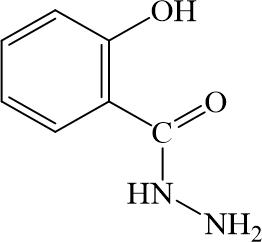
\includegraphics[height=3cm]{media/chem4/image3}
        \caption*{(1a)}
	\end{subfigure}
	\begin{subfigure}{0.58\textwidth}
		\centering
		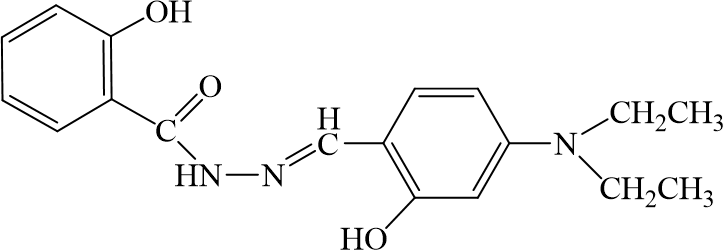
\includegraphics[height=3cm]{media/chem4/image4}
        \caption*{(1b)}
	\end{subfigure}
	
	\begin{subfigure}{0.38\textwidth}
		\centering
		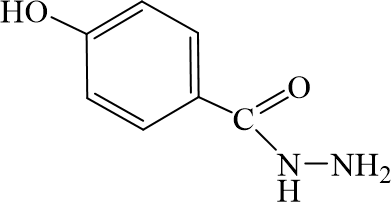
\includegraphics[height=3cm]{media/chem4/image5}
        \caption*{(1c)}
	\end{subfigure}
	\begin{subfigure}{0.58\textwidth}
		\centering
		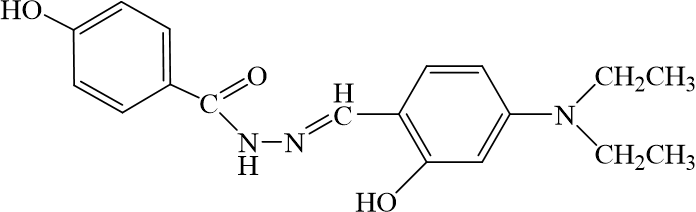
\includegraphics[height=3cm]{media/chem4/image6}
        \caption*{(1d)}
	\end{subfigure}
	\caption*{Рис.1 - Объекты исследования}
\end{figure}


\begin{multicols}{2}
С целью выбора наиболее эффективного комплексообразующего агента из трех
ЦД-нов было выполнено исследование полученных комплексов включений для
системы «циклодекстрин-гидразон» с молярным соотношением (1:1). Эти
исследования проводились методом молекулярного докинга с оценкой
афинности связывания. В качестве объектов исследования выступили
молекулы гидразонов (1а-1d)», а также молекулярные контейнеры -
α-, β- и γ-ЦД («хозяева»). В рамках подготовки молекулярных структур
объектов исследования к докингу их геометрия была первоначально
оптимизирована методом DFT RB3LYP/6-31G CPCM (water) для определения
наиболее устойчивых конформаций и оценки их параметров {[}13-15{]}
(рисунки 2 и 3).
\end{multicols}

\begin{figure}[H]
    \centering
    \begin{subfigure}[t]{0.35\textwidth}
        \centering
        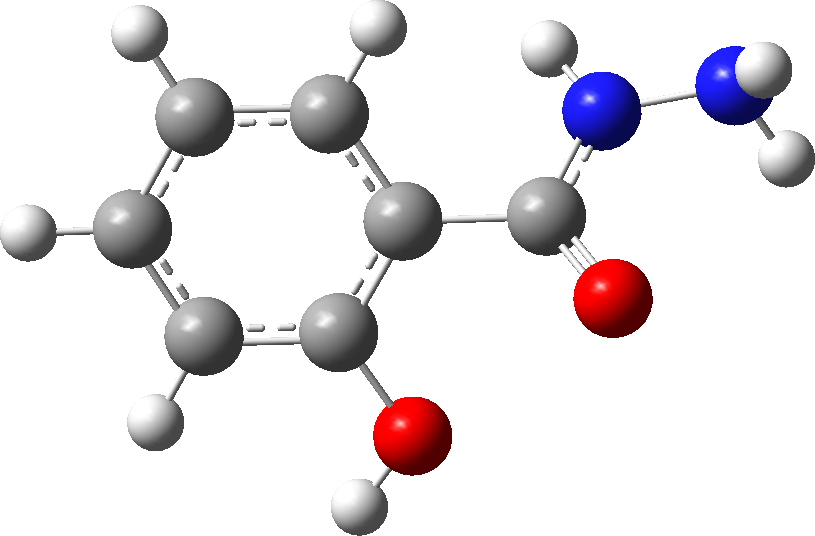
\includegraphics[width=\textwidth, height=4cm]{media/chem2/image31}
        \caption*{1а}
    \end{subfigure}
    \hfill
    \begin{subfigure}[t]{0.55\textwidth}
        \centering
        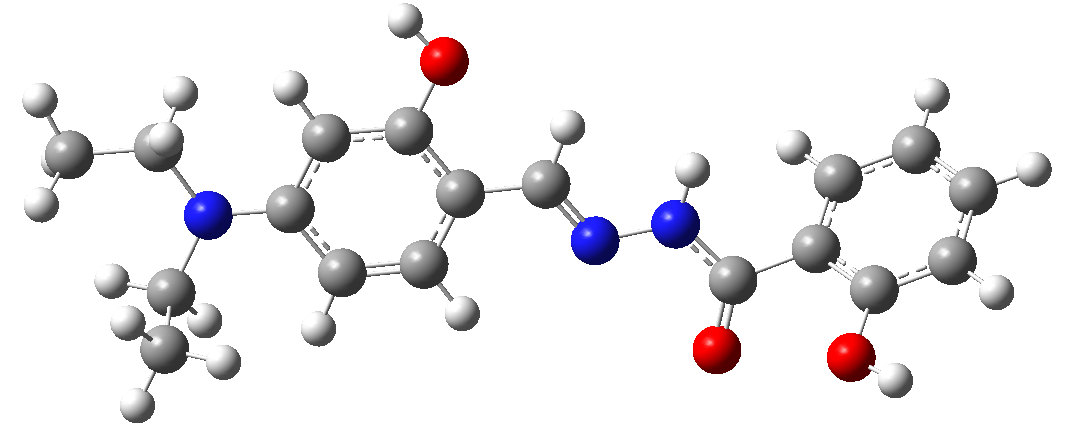
\includegraphics[width=\textwidth, height=4cm]{media/chem2/image32}
        \caption*{1b}
    \end{subfigure}
    
    \begin{subfigure}[t]{0.35\textwidth}
        \centering
        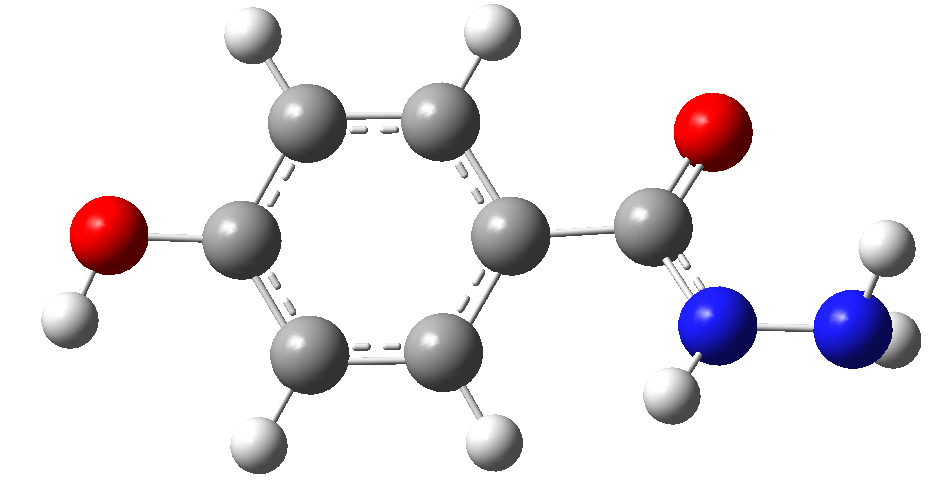
\includegraphics[width=\textwidth, height=4cm]{media/chem2/image33}
        \caption*{1c}
    \end{subfigure}
    \hfill
    \begin{subfigure}[t]{0.55\textwidth}
        \centering
        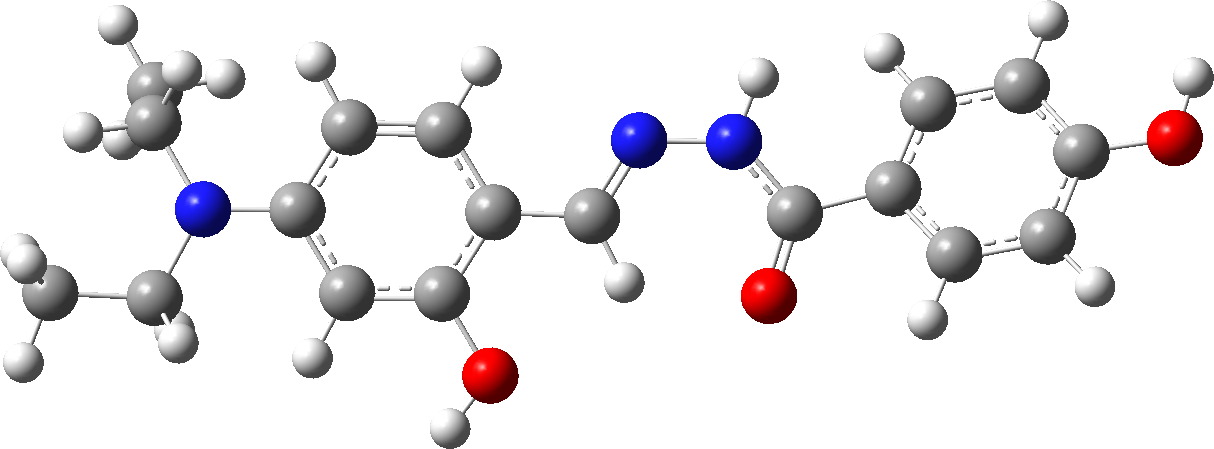
\includegraphics[width=\textwidth, height=4cm]{media/chem2/image34}
        \caption*{1d}
    \end{subfigure}
    \caption*{{\bfseries Рис.2 - Оптимизированные геометрии объектов исследования}}
\end{figure}

\begin{multicols}{2}
Как следует из данных рисунка 2, каркас гидразоновых молекул
характеризуется определенной жесткостью благодаря наличию устойчивых к
конформационной деформации бензольных колец, а также наличию
препятствующей свободному вращению C=N-N-группы. Такая двойственная
природа структуры ЦД (гидрофобность и гидрофильность структуры)
позволяет им включать гидрофобные молекулы-гости внутри себя, улучшая их
растворимость и стабильность в водных растворах. Оптимизированные позы
связывания гидразонов с α-, β- и γ-ЦД показаны на рисунке 3.

Соотношение геометрических параметров молекул гидразонов с размерами
полостей молекул α-, β- и γ-ЦД-нов позволяет предположить наиболее
эффективное связывание с β- и γ-ЦД-нами, так как «контейнер» молекулы
α-ЦД слишком мал для вмещения молекул исследуемых гидразонов. Полученные
в результате оптимизации геометрии объектов исследования были
сконвертированы в *.pdb формат и использованы для выполнения процедуры
молекулярного докинга комплексов включения по типу «контейнер-гость» с
молярным соотношением 1:1 {[}13-15{]}. В качестве молекул «контейнера»
использовались мономеры α-, β- и γ-циклодекстринов, в качестве молекул
«гостей» - молекулы гидразонов. Полученные в результате молекулярного
докинга данные афинности связывания молекул представлены в таблице 1.
\end{multicols}

\begin{longtblr}[
  label = none,
  entry = none,
]{
  width = \linewidth,
  colspec = {Q[240]Q[217]Q[240]Q[217]},
  cells = {c},
  cell{3}{1} = {c=2}{0.456\linewidth},
  cell{3}{3} = {c=2}{0.456\linewidth},
  cell{6}{1} = {c=2}{0.456\linewidth},
  cell{6}{3} = {c=2}{0.456\linewidth},
  cell{7}{1} = {c=4}{0.913\linewidth},
  cell{10}{1} = {c=2}{0.456\linewidth},
  cell{10}{3} = {c=2}{0.456\linewidth},
  cell{13}{1} = {c=2}{0.456\linewidth},
  cell{13}{3} = {c=2}{0.456\linewidth},
  cell{14}{1} = {c=4}{0.913\linewidth},
  cell{17}{1} = {c=2}{0.456\linewidth},
  cell{17}{3} = {c=2}{0.456\linewidth},
  cell{18}{1} = {c=4}{0.913\linewidth},
  hlines,
  vlines,
}
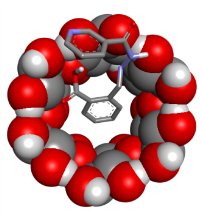
\includegraphics[width=0.18\textwidth,height=0.18\textwidth]{media/chem2/image35} &
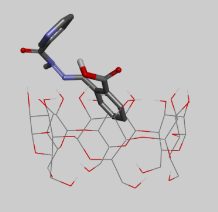
\includegraphics[width=0.18\textwidth,height=0.18\textwidth]{media/chem2/image36} &
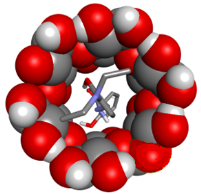
\includegraphics[width=0.18\textwidth,height=0.18\textwidth]{media/chem2/image37} &
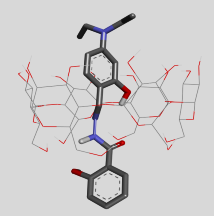
\includegraphics[width=0.18\textwidth,height=0.18\textwidth]{media/chem2/image38}\\
Вид сверху & Вид сбоку & Вид сверху & Вид сбоку\\
$\alpha$-CD с 1a &  & $\alpha$-CD с 1b & \\
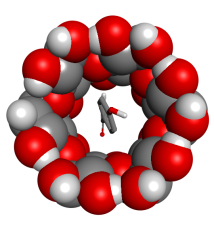
\includegraphics[width=0.18\textwidth,height=0.18\textwidth]{media/chem2/image39} &
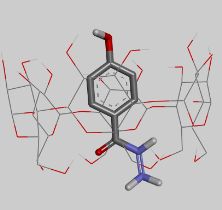
\includegraphics[width=0.18\textwidth,height=0.18\textwidth]{media/chem2/image40} &
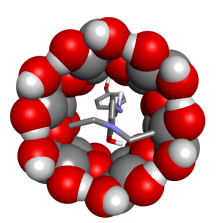
\includegraphics[width=0.18\textwidth,height=0.18\textwidth]{media/chem2/image41} &
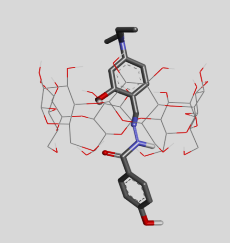
\includegraphics[width=0.18\textwidth,height=0.18\textwidth]{media/chem2/image42}\\
Вид сверху & Вид сбоку & Вид сверху & Вид сбоку\\
$\alpha$-ЦД с 1c &  & $\alpha$-ЦД с 1d & \\
Лучшие позы  с $\alpha$-CDs &  &  & \\
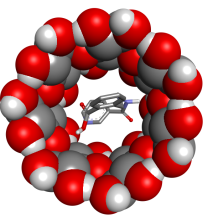
\includegraphics[width=0.18\textwidth,height=0.18\textwidth]{media/chem2/image43} &
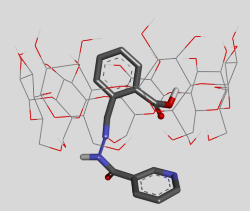
\includegraphics[width=0.18\textwidth,height=0.18\textwidth]{media/chem2/image44} &
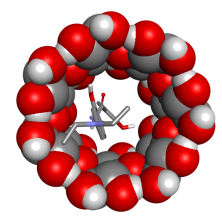
\includegraphics[width=0.18\textwidth,height=0.18\textwidth]{media/chem2/image45} &
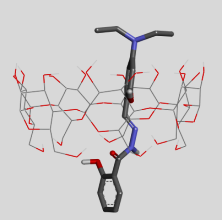
\includegraphics[width=0.18\textwidth,height=0.18\textwidth]{media/chem2/image46}\\
Вид сверху & Вид сбоку & Вид сверху & Вид сбоку\\
$\beta$-ЦД  с  1a &  & $\beta$-ЦД с  1b & \\
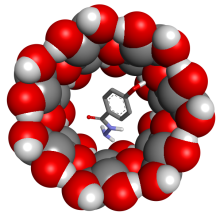
\includegraphics[width=0.18\textwidth,height=0.18\textwidth]{media/chem2/image47} &
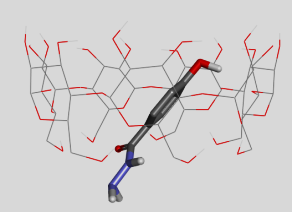
\includegraphics[width=0.18\textwidth,height=0.18\textwidth]{media/chem2/image48} &
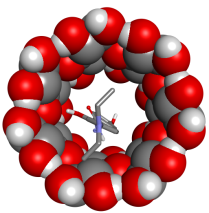
\includegraphics[width=0.18\textwidth,height=0.18\textwidth]{media/chem2/image49} &
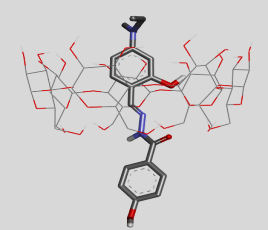
\includegraphics[width=0.18\textwidth,height=0.18\textwidth]{media/chem2/image50}\\
Вид сверху & Вид сбоку & Вид сверху & Вид сбоку\\
$\beta$-ЦД с  1c &  & $\beta$-ЦД с  1d & \\
Лучшие позы  с $\beta$-CDs &  &  & \\
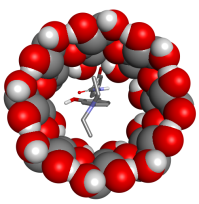
\includegraphics[width=0.18\textwidth,height=0.18\textwidth]{media/chem2/image51} &
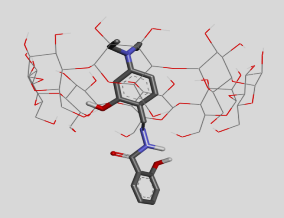
\includegraphics[width=0.18\textwidth,height=0.18\textwidth]{media/chem2/image52} &
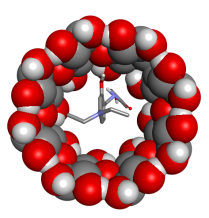
\includegraphics[width=0.18\textwidth,height=0.18\textwidth]{media/chem2/image53} &
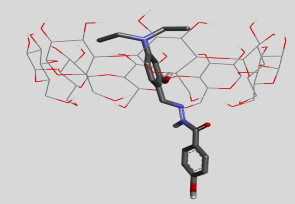
\includegraphics[width=0.18\textwidth,height=0.18\textwidth]{media/chem2/image54}\\
Вид сверху & Вид сбоку & Вид сверху & Вид сбоку\\
$\gamma$-ЦД с 1a &  & $\gamma$-ЦД с 1b & \\
Лучшие позы  с $\gamma$-ЦД &  &  & 
\end{longtblr}
\tcap{Рис.3 - Оптимизированные позы связывания гидразонов с α-, β- и γ-циклодекстринами}

\begin{multicols}{2}
Как следует из представленных в таблице 1 данных, наилучшее связывание
все изучаемые гидразоны проявили с β-ЦД-ном, чуть менее эффективное
связывание в большинстве случаев было продемонстрировано с γ-ЦД-ном, за
исключением гидразонов {\bfseries 1b} и {\bfseries 1c}, которые после β-ЦД
более эффективно взаимодействовали с α-ЦД-ном.
\end{multicols}

\tcap{Таблица 1 - Афинность связывания для комплексов гидразон--циклодекстрин (1:1), ккал/моль}
\begin{longtblr}[
  label = none,
  entry = none,
]{
  cells = {c},
  hlines,
  vlines,
}
Циклодекстрин Гидразон & $\alpha$-CD & $\beta$-CD & $\gamma$-CD\\
1а & -4.2 & -5.0 & -4.5\\
1b & -5.3 & -5.7 & -5.1\\
1c & -5.0 & -5.3 & -4.8\\
1d & -4.2 & -5.7 & -4.3
\end{longtblr}

\begin{multicols}{2}
Наилучшее значение афинности связывания от -5,0 до -5,7 ккал/моль
гидразоны (1а-d) продемонстрировали с β-ЦД-ном. Наихудшее связывание
продемонстрировали гидразоны (1a) и (1d) с α-ЦД-ном,
показав афиннность связывания -4,2 ккал/моль. Достаточно эффективное
взаимодействие гидразонов (1b) и (1c) (афинность связывания
-5,3 и -5,0 ккал/моль соответственно) с α-ЦД-ном, что по-видимому,
обусловлено наличием в них длинного -С-N-N=C- мостика, а также полярных
-С=О и -С-О-Н, обеспечивающих проникновение и закрепление молекулы гостя
в полость хозяина.

Для того чтобы лучше понять возможные режимы связывания исследуемых
гидразонов с предпочтительными ЦД-нами, была выполнена визуализация
наиболее эффективных комплексов включения. Анализ представленных на
рисунке 4 геометрий комплексов гидразон-ЦД показывает, что с α-ЦД-ном
гидразоны (1a) имеют поверхностное связывание, без проникновения
молекулы гостя в полость хозяина, что проявляется в низких значениях
афинности связывания {[}14,15{]}. Во всех остальных случаях гидразоны
демонстрируют частичное или полное проникновение внутрь полости ЦД-нов.
Интересно отметить, что в случае с γ-ЦД-ном, несмотря на проникновение
молекул гидразонов внутрь полости тора, исследуемые гидразоны
демонстрируют менее эффективное связывание чем в случае с β-ЦД-ном, что
обусловлено, по-видимому, несоответствием размера полости тора γ-ЦД
геометрическим параметрам молекул гидразонов - в ряде случаем можно
отметить, как молекула «гостя» буквально «проваливается» сквозь полость
γ-ЦД (рисунок 4).

В целом, моделирование с помощью инструментов молекулярного докинга
позволило выявить β-ЦД как наиболее эффективный комплексообразующий
агент для исследуемых гидразонов. Все исследуемые гидразоны
продемонстрировали наилучшее значение афинности связывания с β-ЦД-ном.
При этом для молекул (1b{\bfseries ), (}1c) комплексообразователем
второго выбора может быть рекомендован α-ЦД, а для остальных - γ-ЦД.

Термическая стабильность образованных комплексов включения гидразидов и
их гидразоновых производных с β-ЦД-ном были исследованы методом
термогравиметрического анализа {[}16{]}. Этот метод позволяет учитывать
изменение массы супрамолекулярных комплексов включением субстратов от
температуры и на основе ее пиков точно определять скорость термического
разложения изучаемых образцов. Кривые, представленные на рисунке 5,
отображают результаты термогравиметрического анализа (ТГА) и
производного термогравиметрического анализа (ДТГ) для различных
образцов: циклодекстрина (ЦД), его физических смесей с гидразоном, а
также комплекса включения ЦД:1d. На ТГА-кривых (рисунок 5,а) показано
изменение массы образцов (ТГ, мг) в зависимости от температуры (°С), а
на ДТГ-кривых (рисунок 5, b) -- скорость изменения массы (мг/мин) по
мере нагревания. Анализ включает три кривые (рисунок 5), обозначенные
как (1) - для ЦД, (2) - для физических смесей ЦД с гидразоном и (3) --
для включения комплекса ЦД:1d. Процесс термической деструкции ЦД, а
также физической смесей ЦД с гидразоном и комплексным включением ЦД:1d
протекает в несколько стадий, сопровождающихся потерями массы,
фиксируемыми на кривых ТГ (термогравиметрический анализ) и ДТГ
(дифференциально-термогравиметрический анализ) {[}16,17{]}.
\end{multicols}

\begin{figure}[H]
    \centering
    \begin{subfigure}[t]{0.3\textwidth}
        \centering
        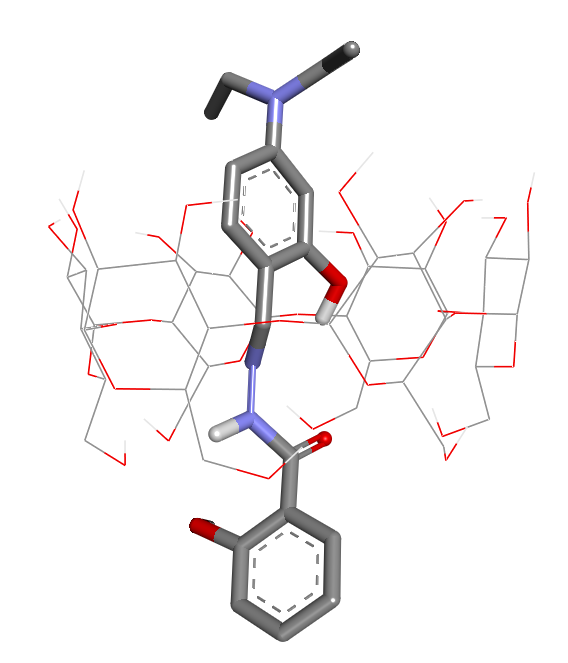
\includegraphics[width=\textwidth, height=4.5cm]{media/chem2/image55}
        \caption*{α-ЦД -- 1b}
    \end{subfigure}
    \begin{subfigure}[t]{0.3\textwidth}
        \centering
        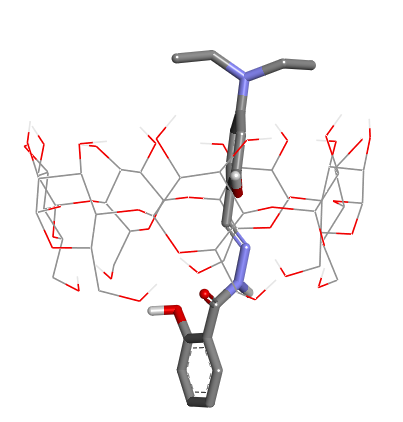
\includegraphics[width=\textwidth, height=4.5cm]{media/chem2/image56}
        \caption*{β-ЦД -- 1b}
    \end{subfigure}
    \begin{subfigure}[t]{0.3\textwidth}
        \centering
        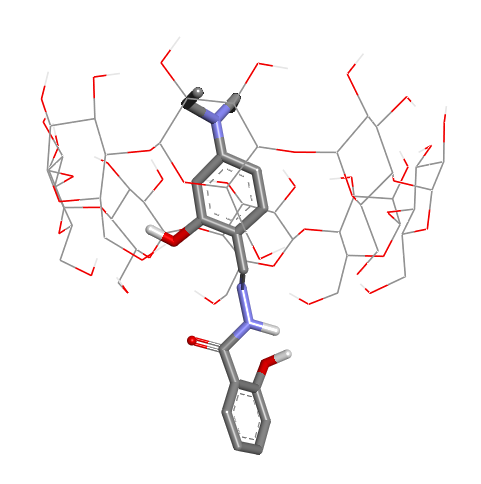
\includegraphics[width=\textwidth, height=4.5cm]{media/chem2/image57}
        \caption*{γ-ЦД -- 1b}
    \end{subfigure}
    \caption*{{\bfseries Рис.4 - Лучшие позы связывания гидразонов 1b с α-, β- и γ-ЦД}}
\end{figure}

\begin{multicols}{2}
Как видно из рисунка 5, для ЦД и физических смесей с гидразоном потеря
массы, связанная с удалением воды, происходит при ∼105°С (7.22 мг, 1.10
мг), тогда как для комплекса включение ЦД:1d − при 102°С (4.52 мг), что
свидетельствует о более сильном связывании воды в комплексе. Это
подтверждается более выраженным низкотемпературным пиком на ДТГ-кривой
(рисунок 5, b), что соответствует эндоэффектам (рисунок 5, III) при
122.84°С и 111.98°С, 161.88°С для 1-го образца (рисунок 5, I) и при
108.73°С для 2-го образца (рисунок 5, II). В интервале температуры
300--345°С (ДСК\textsubscript{max} = 337.18°С) для 1-го образца (ЦД),
333--364°С (ДСК\textsubscript{max} = 349.04°С; 362.35°С) для 3-го
образца (ЦД:1d), а также 303--340°С (ДСК\textsubscript{max} = 332.52°С;
336.98°С) для химических смесей ЦД с гидразоном наблюдаются эндоэффекты,
приводящие к резким потерям масс (таблица 2).
\end{multicols}

\tcap{Таблица 2 - Данные термограмм комплексов β-ЦД, физические смеси ЦД с гидразоном и комплекса включения ЦД:1d}

\begin{longtblr}[
  label = none,
  entry = none,
]{
  width = \linewidth,
  colspec = {Q[406]Q[98]Q[238]Q[194]},
  cells = {c},
  hlines,
  vlines,
}
Параметр & β-ЦД & Физическая
				смесь ЦД с гидразоном & Комплекс
				включения ЦД:1d\\
Температура
				начала потери массы, °С & 105°С & 90°С & 102°С\\
Температура
				максимальная скорость разложения
				(ДТГ max),
				°С & 336°С & 346°С & 330°С\\
Потеря
				массы на начальном этапе (до 150°С), \% & 7.22
				мг & 1.10
				мг & 4.52
				мг\\
Температурный
				диапазон основных разложений, °С & 305–376°С & 305–400°С & 305–393°С\\
Остаточная
				масса при 600°С, \% & 68.63
				мг & 69.58
				мг & 53.33
				мг\\
Эндотермические
				эффекты (наличие, температура), °С & {
				211.88°С
				\\
				337.18°С
			} & {
				322.52°С
				\\
				336.98°С
			} & {
				241.89°С
				\\
				322.66°С
				\\
				349.57°C
			}\\
Удержание
				воды (по потерям при \textasciitilde{}100°C),
				мг & 4.53
				мг & 0.55
				мг & 2.51
				мг
\end{longtblr}

\begin{figure}[H]
	\centering
	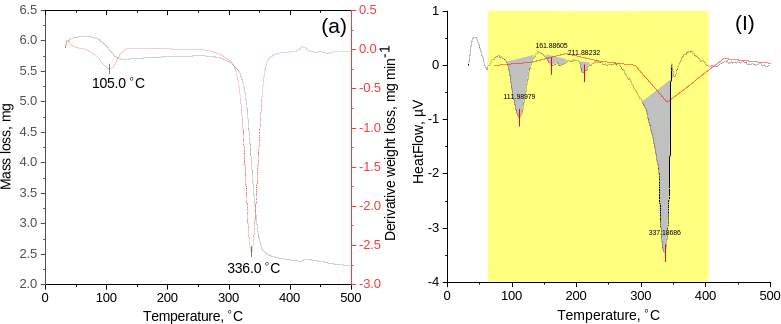
\includegraphics[width=0.74\textwidth]{media/chem2/image58}
\end{figure}
\begin{figure}[H]
	\centering
	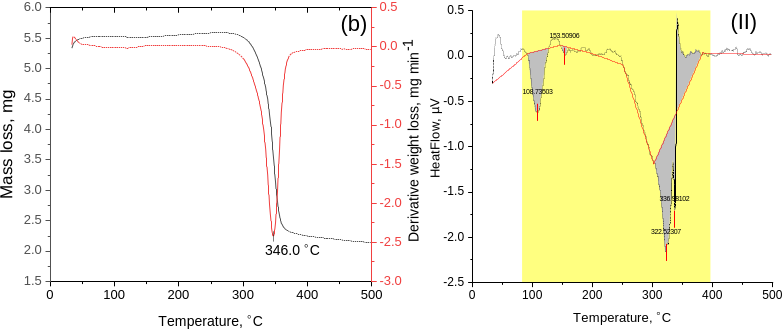
\includegraphics[width=0.74\textwidth]{media/chem2/image59}
\end{figure}
\begin{figure}[H]
	\centering
	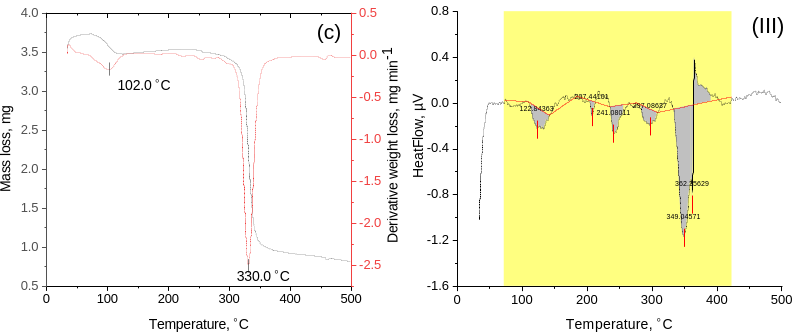
\includegraphics[width=0.74\textwidth]{media/chem2/image60}
	\caption*{Рис.5 -Термические кривые: (a) − ЦД (I), (b) − физической смеси ЦД с гидразоном (II) и (c) − комплекса включения ЦД:1d (III)}
\end{figure}

\begin{multicols}{2}
Эти изменения приводят к началу процесса термической деструкции, при
этом ТГ- и ДТГ-кривые показывает, что последовательное разложение
комплекса включение ЦД:1d начинается при более низкой температуре
(ДТГ\textsubscript{max} = 330°С), чем для физической смеси ЦД с
гидразоном (ДТГ\textsubscript{max} = 346°С) {[}16-18{]}. Однако
одновременно наблюдается, что комплекс включения ЦД:1d способствует
усилению соединения воды в ЦД, но уменьшает термическую стабильность
самого ЦД (таблица 2).

{\bfseries Выводы.} Гидразид--гидразоновые производные бензойной кислоты
составляют основу многих лекарственных препаратов и проявляют широкий
спектр биологических активностей. В результате проведенных исследований
получены новые водорастворимые капсулированные производные гидразонов 2-
и 4-гидроксибензойной кислоты с β- и γ-циклодекстринами. Исследования
полученных супракомплексов показало, что в обоих случаях образуются
комплексы включения субстратов с молекулами комплексообразователя.
Образование комплексообразования субстратов c рассмотренными
комплексообразователями протекает в одинаковой степени с участием как
внутренних протонов циклодекстриновой полости, так и расположенных на
внешней поверхности конического конуса с образованием смешанных
комплексов включений. Соотношение геометрических параметров молекул
гидразонов с размерами полостей молекул α-, β- и γ-циклодекстринов
позволяет предположить наиболее эффективное связывание с β- и
γ-циклодекстринами, так как внутренний размер молекулы α-циклодекстрина
слишком мал для вмещения молекул исследуемых гидразонов. Результаты
анализа термодеструкции комплекса включения свидетельствуют о повышении
термостабильности молекулы ЦД при включении в его полость биологически
активного компонента.

\emph{{\bfseries Финансирование:} Научно-исследовательская работа
осуществлена в рамках ПЦФ} BR24992921 \emph{Комитета науки Министерства
науки и высшего образования Республики Казахстан}.
\end{multicols}

\begin{center}
{\bfseries References}
\end{center}

\begin{references}
1. Popiolek L. Hydrazide--hydrazones as potential antimicrobial
agents:overview of the literature since 2010 // Med Chem. Res., 2016. -
№ 26(2). - Р.287-301. DOI 10.1007/s00044-016-1756-y.

2. Papakonstantinou-Garoufalias S., Pouli N., Marakos P.,
ChytyroglouLadas A. Synthesis antimicrobial and antifungal activity of
some new 3 substituted derivatives of
4-(2,4-dichlorophenyl)-5-adamantyl-1H-1,2,4-triazole // Farmaco.- 2002.
- № 57. - Р.973-977. DOI 10.1016/s0014-827x(02)01227-2

3. Belyaeva E.R., Yu V., Myasoedova N.M., Ishmuratova G., Ishmuratov Yu.
// Russian Journal of Bio\-organic Chemistry.- 2022. - № 48. - Р.
1123. DOI 10.1134/S1068162022060085

4. Kaymakçıoğlu B.K., Rollas S. Synthesis, characterization and
evaluation of antituberculosis activity of some hydrazones // Farmaco.
2002. - № 57. -Р.595-599. DOI: 10.1016/s0014-827x(02)01255-7

5. Melnyk P., Leroux V., Sergheraert C., Grellier P. Design, synthesis
and in vitro antimalarial activity of an acylhydrazone library//Bioorg.
Med. Chem. Lett.- 2006.-№ 16.- Р.31-35.

DOI 10.1016/j.bmcl.2005.09.058

6. Todeschini A.R., Miranda A.L.P., Silva K.C.M., Parrini S.C., Barreiro
E.J. Synthesis and evalution of analgesic, anti-inflammatory and
antiplatelet properties of new 2-pyridyalhydrazone derivatives // Eur.
J. Med. Chem.- 1998.- № 33.- Р.189-199. DOI
10.1016/s0223-5234(98)80008-1

7. Rollas S., Gulerman N., Erdeniz H. Synthesis and antimicrobial
activity of some new hydrazones of 4-fluorobenzoic acid hydrazide and
3-acetyl-2,5-disubstituted-1,3,4-oxadiazolines // Farmaco.- 2002. - №
57. -Р.171-174. DOI 10.1016/s0014-827x(01)01192-2

8. Zhou P.P., Sun X.B., Qiu W.Y. Nicotinic acid and its derivatives:
synthetic routes, crystal forms and polymorphs//Current drug discovery
technologies.-2014 .- № 11. -Р.97.

DOI 10.2174/1570163811666140225152610

9. Huang R., Jiang N, Geng X., Lin J., Zhou G.Q. et al. Fibroscan
improves the diagnosis sensitivity of liver fibrosis in patients with
chronic hepatitis B. //~Experimental and Therapeutic Medicine.- 2016.-№
11. - Р.
1673-1677.~DOI~\href{http://doi.org/10.3892/etm.2016.3135}{10.3892/etm.2016.3135}~

10. Jansook P., Ogawa N., Loftsson T. Cyclodextrins: structure,
physicochemical properties and pharma\-ceutical
applications//International Journal of Pharmaceutics .- 2018.-№
5. - Р.535.

DOI 10.1016/j.ijpharm.2017.11.018.

11. Pinho E., Soares G., Henriques M. Cyclodextrin modification of gallic
acid in vitro antibacterial activity // Journal of Inclusion Phenomena
and Macrocyclic Chemistry .- 2015.-№ 81. - Р.205-2014. DOI
10.1007/s10847-014-0449-8

12. Fazylov S.D., Satpaeva Zh.B., Nurkenov O.A., Bakirova R.E.,
Sviderskij A.K., Mendibaeva A.Zh. Poluchenie vodorastvorimyh kompleksov
vkljuchenij gidrazidovo-ip-gidroksibenzojnyh kislot i ih gidra\-zonovyh
proizvodnyh//Vestnik KazUTB.-2024.-№ 3(24).- R.250-259

DOI 10.58805/kazutb.v.3.24-501.{[}in Russian{]}

13. Nurkenov O.A., Fazylov S.D., Satpaeva Zh., Seilkhanov T.M.,
Turdybekov D.M., Mendibaeva A.Zh., Akhmetova S.B., Shulgau Z.T.,
Alkhimova L.E., Kulakov I.V. Synthesis, structure and biological
activity of hydrazones derived from 2- and 4-hydroxybenzic acid
hydrazides // Chemical Date Collections.- 2023. - № 48. - Р.1-13. DOI
10.1134/s1070363219100098~

14. Gunsteren W. F. van, Oostenbrink C. Methods for Classical-Mechanical
Molecular Simulation in Chemistry: Achievements, Limitations,
Perspectives~ // Journal of Chemical Information and Modeling.- 2024. -
№ 64(16). -Р.6281. DOI10.1021/acs.jcim.4c00823

15. Dennington R., Keith T., Millam J. Gauss View // Semichem Inc.,
Shawnee Mission, KS.- Environment\-ally Friendly Room Temperature
Synthesis of 1-Tetralone over Layered Double Hydroxide-Hosted
Sulph\-onato-Salen-Nickel(II) Complex.2016. -№ 6.- P.9-22
DOI 10.4236/gsc.2023.131002

15. Brunk E., Rothlisberger U., Mixed Quantuan Molecular
mechanical/molecular dinamics Simulations of biological systems in
ground and electronically excited
states//Chem.Rev.-2015.-Vol.115(12).-P.-6217-6263. DOI 10.1021/cr50062b

16. Castronuovo G., Niccoli M. Thermodynamics of inclusion complexes of
natural and modified cyclodex\-trins with acetylsalicylic acid and
ibuprofen in aqueous solution at 298 K // Thermochimica Acta.- 2013. -
Vol.557. - Р.44-49. DOI 10.1016/j.tca.2013.01.037~

17. Сastronuovo G., Niccoli M. Thermodynamics of inclusion complexes of
natural and modified cyclodex\-trins with propranolol in aqueous solution
at 298 K // Bioorganic and Medical Chemistry.- 2006. - Р.3883-3887. DOI
10.1016/j.bmc.2006.01.052

18. Qvist J., Halle B. Thermal signature of hydrophobic hydration
dinamics // American Chemical Society.- 2008. -Vol.130(31).-
Р.10345-10353. DOI: 10.1021/ja802668w
\end{references}

\begin{authorinfo}
\hspace{1em}\emph{{\bfseries Сведения об авторах}}  

Мулдахметов З.М. — академик НАН РК, доктор химических наук, профессор,
директор Института органического синтеза и углехимии Республики
Казахстан, Караганда, Казахстан, e-mail: iosu@mail.ru;

Фазылов С.Д. — доктор химических наук, профессор, главный научный
сотрудник Института органического синтеза и углехимии, Караганда,
Казахстан, e-mail: iosu8990@mail.ru;

Нуркенов О.А. — доктор химических наук, профессор, заведующий
лабораторией Синтез биологически активных веществ Института
органического синтеза и углехимии, Караганда, Казахстан, e-mail:
nurkenov\_oral@mail.ru;

Сарсенбекова А.Ж. — доктор PhD, ведущий научный сотрудник
Карагандинского университета имени Е.А. Букетова, Караганда,
Казахстан, e-mail: chem\_akmaral@mail.ru;

Пустолайкина И.А. — кандидат химических наук, ассоциированный
профессор, ведущий научный сотрудник Карагандинского университета
имени Е.А. Букетова, Караганда, Казахстан, e-mail:
ipustolaikina@gmail.com;

Сатпаева Ж.Б. — старший преподаватель кафедры органической химии и
полимеров Карагандинского университета им. Е.А. Букетова, Караганда,
Казахстан, e-mail: satpaeva\_zh@mail.ru;

Бакирова Р.Е. — доктор медицинских наук, профессор кафедры внутренних
болезней Медицинского университета Караганды, Караганда, Казахстан,
e-mail: bakir15@mail.ru;

Нурмаганбетов Ж.С. — кандидат химических наук, ассоциированный
профессор Института органического синтеза и углехимии, Караганда,
Казахстан, e-mail: nzhangeldy@yandex.ru;

Мусина Г.Н. — кандидат химических наук, доцент, Карагандинский
технический университет им. А. Сагинова, Караганда, Казахстан, e-mail:
gulnaz\_musina@mail.ru;

Сыздыков А.К. — младший научный сотрудник Института органического
синтеза и углехимии, Караганда, Казахстан, e-mail:
ardak.syzdykov.96@inbox.ru.

\hspace{1em}\emph{{\bfseries Information about the authors}}  

Muldakhmetov Z.M. — Academician of the National Academy of Sciences of
the Republic of Kazakhstan, Doctor of Chemical Sciences, Professor,
Director of the Institute of Organic Synthesis and Coal Chemistry of
the Republic of Kazakhstan, Karaganda, Kazakhstan, e-mail:
iosu@mail.ru;

Fazylov S.D. — Doctor of Chemical Sciences, Professor, Chief
Scientific Associate of the Institute of Organic Synthesis and Coal
Chemistry, Karaganda, Kazakhstan, e-mail: iosu8990@mail.ru;

Nurkenov Oral A. — Doctor of Chemical Sciences, Professor, Head of the
Laboratory of Synthesis of Biologically Active Substances, Institute
of Organic Synthesis and Coal Chemistry, Karaganda, Kazakhstan,
e-mail: nurkenov\_oral@mail.ru;

Sarsenbekova A.Zh. — PhD in Chemistry, Leading Researcher,
E.A. Buketov Karaganda University, Karaganda, Kazakhstan, e-mail:
chem\_akmaral@mail.ru;

Pustolaykina I.A. — Candidate of Chemical Sciences, Associate
Professor, Leading Researcher, E.A. Buketov Karaganda University,
Karaganda, Kazakhstan, e-mail: ipustolaikina@gmail.com;

Satpaeva Zh.B. — Senior Lecturer of the Department of Organic
Chemistry and Polymers, E.A. Buketov Karaganda University, Karaganda,
Kazakhstan, e-mail: satpaeva\_zh@mail.ru;

Bakirova R.E. — Doctor of Medical Sciences, Professor of Internal
Medicine Department, Medical University of Karaganda, Karaganda,
Kazakhstan, e-mail: bakir15@mail.ru;

Nurmaganbetov Zh.S. — Candidate of Chemical Sciences, Associate
Professor, Institute of Organic Synthesis and Coal Chemistry,
Karaganda, Kazakhstan, e-mail: nzhangeldy@yandex.ru;

Musina G.N. — Candidate of Chemical Sciences, Associate Professor,
A. Saginov Karaganda Technical University, Karaganda, Kazakhstan,
e-mail: gulnaz\_musina@mail.ru;

Syzdykov A.K. — Junior Researcher, Institute of Organic Synthesis and
Coal Chemistry, Karaganda, Kazakhstan, e-mail:
ardak.syzdykov.96@inbox.ru.
\end{authorinfo}
